\documentclass[t,12pt]{beamer}

\usepackage{amsmath}
\usepackage{amsfonts}
\usepackage{amssymb}
\usepackage{amsthm}
\usepackage{mathrsfs}
\usepackage{dsfont}
\usepackage[utf8x]{inputenc}
\usepackage[labelfont=bf,justification=justified]{caption}
\usepackage{subcaption}
\usepackage{fixltx2e}
\usepackage{setspace}
\usepackage{arydshln}
\usepackage{xcolor}
\usepackage{tikz}
\usepackage{chngpage}
\usepackage{comment}
\usetikzlibrary{shapes,arrows}
\tikzstyle{block} = [rectangle, draw, fill=blue!20, 
    text width=5em, text centered, rounded corners, minimum height=4em]
\tikzstyle{line} = [draw, -latex']

\usetheme{Emory}
\makeatletter
\setbeamertemplate{footline}
{
  \leavevmode%
  \hbox{%
  \begin{beamercolorbox}[wd=.333333\paperwidth,ht=2.25ex,dp=1ex,center]{author in head/foot}%
    \usebeamerfont{author in head/foot}\insertshortauthor~~\beamer@ifempty{\insertshortinstitute}{}{\insertshortinstitute}
  \end{beamercolorbox}%
  \begin{beamercolorbox}[wd=.333333\paperwidth,ht=2.25ex,dp=1ex,center]{title in head/foot}%
    \usebeamerfont{title in head/foot}\insertshorttitle
  \end{beamercolorbox}%
  \begin{beamercolorbox}[wd=.333333\paperwidth,ht=2.25ex,dp=1ex,right]{date in head/foot}%
    \usebeamerfont{date in head/foot}\insertshortdate{}\hspace*{2em}
    \insertframenumber{} / \inserttotalframenumber\hspace*{2ex} 
  \end{beamercolorbox}}%
  \vskip0pt%
}
\makeatother

\setbeamerfont{frametitle}{size=\large}
\setbeamertemplate{navigation symbols}{}

\titlegraphic{\includegraphics[width=0.3\textwidth]{/home/william/Emory.png}}

\begin{document}

\title[Volatility modeling]{Volatility modeling}
\author{\vspace{0.35in} \\ {\fontfamily{ppl}\selectfont William Mann} \vspace{-0.35in}}

\date{}
\maketitle

\begin{frame}[c]{Motivation: Time-varying, persistent volatility}
\centerline{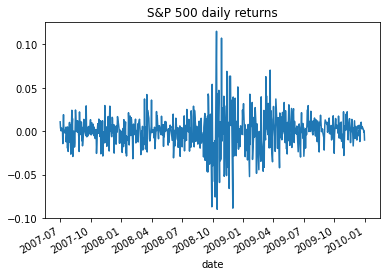
\includegraphics[width=0.6\linewidth]{crisis_volatility.png}}
\begin{itemize}
\item Many datasets, especially financial data, exhibit time-varying and persistent volatility.
We'd like to model this for many reasons, especially risk management.
\item Note that it is really the \emph{persistence} that is important to model.
\end{itemize}
\end{frame}

\begin{frame}[c]{Outline}
\begin{itemize}
\item Engle's ARCH-LM test for persistence in volatility.
\medskip
\item Modeling persistence in volatility with GARCH.
\medskip
\item Application: Value-at-risk calculations.
\end{itemize}
\medskip
A general theme is to use $r_t^2$ as an estimate of $\sigma_t^2$, and adapt the tools that we already know from prior weeks around this idea.
\end{frame}


\begin{frame}[c]{Engle's ARCH-LM test for persistence in volatility}
When $\sigma_t^2$ is high, is $\sigma_{t+1}^2$ likely to also be high?
\begin{itemize}
\item This is like checking for time-series effects in any dataset.
\item Could we just apply one of our existing tests to data on $\sigma_t^2$?
\item The major problem is, you can't directly measure $\sigma_t^2$.
\item Instead, focus on $r_t^2$ as an indirect measure.
\end{itemize}
\medskip
The standard test is known as \emph{Engle's test} or the \emph{ARCH-LM} test.
\begin{itemize}
\item Run the following regression: $r_t^2 = \alpha + \beta r_{t-1}^2 + \varepsilon_t$
\item Under the null of no persistence in $\sigma_t^2$, we have $N \times R^2 ~ \sim \chi^2$.
\item Implemented in statsmodels with the \emph{het\_arch} command.
\item You can also extend the regression to include $p$ lags of $r_t^2$.
\\ Then the test statistic is asymptotically $\chi^2(p)$.
\\ By default, het\_arch uses a lag of $\sqrt{T}$, rounding down. %
\end{itemize}
\end{frame}

\begin{frame}[c]{Modeling persistent volatility: Moving average}
One popular way to measure volatility over time is through a moving average.
This works much like the moving average from week 1.
\\ \bigskip
But, a complication is that you cannot actually measure volatility at any point in time.
Instead, the moving-average estimate of volatility is based on an average of $r_t^2$ terms:
$$
\sigma_{t,CMA}^2 \quad = \quad \frac{1}{m} \left( \frac{1}{2} \, r_{t-m}^2 + r_{t-m+1}^2 + \dots + r_{t+m-1}^2 + \frac{1}{2} \, r_{t+m}^2 \right)
$$
This is a fast and easy way to describe and plot volatility over time.
\end{frame}

\begin{frame}[c]{Modeling persistent volatility: EWMA}
\begin{itemize}
\item EWMA stands for Exponentially Weighted Moving Average.
\medskip
\item The basic idea is like exponential smoothing from week 2.
\medskip
\item You choose a smoothing parameter $\alpha$, and an initial $\sigma_0^2$, 
\\ which is often the sample value from the first few observations.
\medskip
\item Then update the values of $\sigma_t$ following the formula:
$$
\sigma_{t+1}^2 \quad = \quad \alpha \times r_t^2 \, + \, (1-\alpha) \times \sigma_t^2
$$
\item Higher $\alpha$ moves you close to just estimating tomorrow's volatility with today's $r^2$.
Lower $\alpha$ gives smoother results that react more slowly to changes, for better and for worse.
\end{itemize}
\end{frame}

\begin{frame}[c]{Smoothing vs model-based approaches}
\begin{itemize}
\item We can make some of the same comments here that we did after we covered Holt-Winters forecasting:
\item Smoothing-based approaches give an easy and effective way to describe the data and build accurate forecasts. 
\\ If that is our only goal, they are likely to be good enough.
\item But these approaches will break down as we move our attention to other goals like building confidence intervals, or understanding relationships between different series.
\item At some point we have to adopt the \emph{model-based} approach that is more standard in statistics.
\item Before, this led us to ARMA.  Here it leads us to a set of volatility models that will be our main focus.
\end{itemize}
\end{frame}

\begin{frame}[c]{Modeling persistence in volatility: ARCH}
The simplest and oldest volatility model is called ARCH
\\ (which stands for ``\textbf{A}uto\textbf{R}egressive \textbf{C}onditional \textbf{H}eteroskedasticity'')
\vspace{-0.1in}
\begin{align*}
y_t &= \mu + u_t \quad , \quad u_t \sim \mathscr{N}(0,\sigma_t^2)
\\
\sigma_t^2 &= \omega + \alpha u_{t-1}^2
\end{align*}
\begin{itemize}
\vspace{-0.3in}
\item The first line could be replaced with any ARMA model for $y_t$.
However, in practice volatility modeling is most important in situations where there probably is no predictability in $y_t$. %
\item The important thing is the second line:
When today's (squared) error is large, tomorrow's error has larger variance, through $\alpha$.
\item More generally, an ARCH(q) model includes $q$ lags of $u_t^2$.
\\ The above model is an ARCH(1).
\item ARCH models are typically estimated by MLE.
\end{itemize}
\end{frame}

\begin{frame}[c]{Modeling persistence in volatility: GARCH}
In practice, ARCH models have generally been replaced by GARCH
\\ (``\textbf{G}eneralized \textbf{A}uto\textbf{R}egressive \textbf{C}onditional \textbf{H}eteroskedasticity'')
\vspace{-0.1in}
\begin{align*}
y_t &= \mu + u_t \quad , \quad u_t \sim \mathscr{N}(0,\sigma_t^2)
\\
\sigma_t^2 &= \omega + \alpha u_{t-1}^2 + \beta \sigma_{t-1}^2
\end{align*}
\begin{itemize}
\vspace{-0.3in}
\item The new thing compared to ARCH is the $\beta \sigma_{t-1}^2$ term.
\\ This extra flexibility greatly improves the model performance.
\item This general category of models is called GARCH(p,q), where
\begin{itemize}
\item $p$ is the number of lags of $\sigma_t^2$,
\item $q$ is the number of lags of $u_t^2$,
\end{itemize}
The above model is a GARCH(1,1). 
\\ In this class we will only look at ARCH(1) and GARCH(1,1).
\item Again, GARCH models are typically estimated by MLE.
\end{itemize}
\end{frame}

\begin{frame}[c]{Finding a good model for volatility in the data}
\begin{itemize}
\item Decide on an ARMA model for $y$ (often just $y_t = \mu + u_t$).
\\ In the first step, don't yet model any volatility effects.
\smallskip
\item Estimate the model, apply Engle's ARCH-LM test to the sample residuals $\hat{u}_t$, and examine ACF and PACF plots of $\hat{u}_t^2$.
\smallskip
\item If the test rejects, or you see important patterns in the plots, add a simple ARCH or GARCH specification to your model.
\smallskip
\item Apply Engle's test to the \emph{standardized} residuals $\hat{u}_t / \hat{\sigma}_t$, 
\\ where $\hat{\sigma}_t$ are the model's estimates of volatility over time 
\\ (labeled as conditional\_volatility in Python's ARCH results).
\\ And plot the ACF and PACF of the squared values $(\hat{u}_t / \hat{\sigma}_t)^2$.
\smallskip
\item Add just enough ARCH and GARCH terms, so that the test fails to reject and you don't see important patterns in the plots.
\end{itemize}
\end{frame}

\begin{frame}[c]{Application: Value-at-risk (VAR)}
\begin{itemize}
\item The \textbf{value-at-risk} (VAR) of a portfolio is a percentile of its return distribution over some specified amount of time.
\medskip
\item For example, the 10-day, 5\% value-at-risk is the 5th percentile of the distribution of returns over the next 10 days.
\begin{itemize}
\smallskip
\item To be more precise, it is the \emph{absolute value} of this number, 
\\ because we are usually thinking about low percentiles (losses).
\end{itemize}
\medskip
\item Example: If the 10-day, 5\% VAR is 8\%, we would say you have a 5\% chance of \emph{losing more than 8\%} over the next 10 days.
\begin{itemize}
\smallskip
\item It is also common to express VAR in dollar terms: 
\\ If your portfolio is worth \$1m, and the 10-day 5\% VAR is 8\%, 
\\ then you have a 5\% chance of losing more than \$80k.
\end{itemize}
\end{itemize}
\end{frame}

\begin{frame}[c]{Calculating VAR from a normal distribution}
\begin{itemize}
\item Suppose you have daily return data ending at time $T$,
\\ and you want to know the $\alpha$ \% VAR over the next $K$ days.
\smallskip
\item Let's use $r_{T \to T+K}$ to label the return over the next $K$ days.
\\ The calculation is easy, if we know the \emph{distribution} of $r_{T \to T+K}$.
\smallskip
\item We will use log returns, so $r_{T\to T+K} = r_{T+1} + r_{T+2} + ... + r_{T+K}$.
\smallskip
\item Assume that each day's log return follows a normal distribution.
\\ \hfill {\footnotesize (This is not critical, but it also is not a bad approximation.)}
\smallskip
\item Then $r_{T \to T+K}$ is also normal (a sum of normal variables).
\\ If we can find its mean $\mu_{T \to T+K}$ and its volatility $\sigma_{T \to T+K}$,
\\ then the VAR is just $\mu_{T \to T+K}$ minus a multiple of $\sigma_{T \to T+K}$.
\begin{itemize}
\item A 5\% VAR is approximately $\mu_{T \to T+K} - 1.645\times\sigma_{T \to T+K}$.
\end{itemize}
\end{itemize}
\end{frame}

\begin{frame}[c]{Calculating $\mu_{T \to T+K}$ from daily data}
\begin{itemize}
\item We typically assume there is no predictability in stock returns. 
\medskip
\item Then $\mu_{T \to T+K} = K \times \mu$, where $\mu$ is the average \emph{one-day} return.
\\ \medskip This follows from:
$$
\mathbb{E}[r_{T \to T+K}] = \mathbb{E}[r_{T+1}] + \mathbb{E}[r_{T+2}] + ... + \mathbb{E}[r_{T+K}] = \underbrace{\mu + \mu + ... + \mu}_{\text{$K$ times}}
$$
\item If you \emph{do} think there is predictability in returns, you can just fit a model such as ARMA and forecast in the standard way. 
\\ But in practice, this is not likely to give you meaningful results.
\end{itemize}
\end{frame}

\begin{frame}[c]{Calculating $\sigma_{T \to T+K}$, ignoring predictability in $\sigma$}
\begin{itemize}
\item As in the previous slide, let's start with the simplest case,
\\ where we just assume that $\sigma$ is completely unpredictable.
\begin{itemize}
\medskip
\item (But to be clear, the whole point of this topic is that this is \emph{not} the appropriate approach, and will give us misleading results.) %
\end{itemize}
\medskip
\item In this case, $\sigma_{T \to T+K} = \sqrt{K} \times \sigma$, where $\sigma$ is one-day volatility.
This follows from %
\end{itemize}
\begin{align*}
&\text{Var}(r_{T \to T+K}) = \text{Var}(r_{T+1} + r_{T+2} + ... + r_{T+K})
\\ &\quad = \text{Var}(r_{T+1}) + ... + \text{Var}(r_{T+K}) = \underbrace{\sigma^2 + ... + \sigma^2}_{\text{$K$ times}} = K \times \sigma^2
\end{align*}
Then the $K$-day, 5\% VAR would be $\quad K \times \mu \quad - \quad 1.645 \times \sqrt{K} \times \sigma$.
\end{frame}

\begin{frame}[c]{Calculating $\sigma_{T \to T+K}$, modeling predictability in $\sigma$}
\begin{itemize}
\item Revisit the previous calculation. Now suppose $\sigma$ is predictable. %
\smallskip
\item The first step from before is still correct:
\begin{align*}
\text{Var}(r_{T \to T+K}) &= \text{Var}(r_{T+1} + r_{T+2} + ... + r_{T+K})
\\ &\quad = \text{Var}(r_{T+1}) + \text{Var}(r_{T+2}) + ... + \text{Var}(r_{T+K})
\end{align*}
This is still correct because daily returns are uncorrelated.
\smallskip
\item Now replace each $\text{Var}(r)$ with a \emph{forecast} of that day's variance.
\begin{itemize}
\smallskip
\item Before, we assumed that variance/volatility were unpredictable, 
so our forecast for each day was just the one-day variance $\sigma^2$.
\smallskip
\item Now, we instead use forecasts from a GARCH model.
\end{itemize}
\end{itemize}
\end{frame}

\begin{frame}[c]{How to build volatility forecasts from a GARCH model}
\begin{itemize}
\item Suppose you have chosen and estimated a GARCH model, as described earlier.
Then, you can forecast future values of $\sigma^2$ following a similar approach as with ARMA models.
\smallskip
\item In statsmodels, the forecast() function will do this for you. 
\\ Let's understand how it works.
\smallskip
\item For example, suppose your model was GARCH(1,1).
\\ This means you specified that $\sigma_t^2 = \omega + \alpha u_{t-1}^2 + \beta \sigma_{t-1}^2$,
\\ and you now have estimates of all these things up to time $T$.
\smallskip
\item Your first forecast $\sigma_{T+1}^2$ is just $\hat{\omega} \, + \, \hat{\alpha} \, \hat{u}_T^2 \, + \, \hat{\beta} \, \hat{\sigma}_T^2$.
\begin{itemize}
\item In statsmodels, $\hat{\omega}$, $\hat{\alpha}$, and $\hat{\beta}$ are reported in ``params'';
\\ $\hat{u}$ is in ``resid,'' and $\hat{\sigma}$ is in ``conditional\_volatility''.
\end{itemize}
\smallskip
\item What about the later forecasts? See next slide...
\end{itemize}
\end{frame}

\begin{frame}[c]{Forecasting volatility with a GARCH model (2)}
What is your forecast of $\sigma_{T+2}^2$?
\begin{itemize}
\smallskip
\item The model says $\sigma_{T+2}^2 = \omega + \alpha u_{T+1}^2 + \beta \sigma_{T+1}^2$.
\smallskip
\item We can use the same estimates of $\omega$, $\alpha$, and $\beta$ as we did before, 
\\ and for $\sigma_{T+1}^2$ we substitute the forecast from the previous slide.
\smallskip
\item But what about $u_{T+1}^2$? Although our best forecast of $u_{T+1}$ is zero, our best forecast of its \emph{squared} value is its variance $\sigma_{T+1}^2$.
\\ So we substitute the forecast from the previous slide there too!
\smallskip
\item This means our forecast of $\sigma_{T+2}^2$ is $\hat{\omega} + (\hat{\alpha} + \hat{\beta}) \times \hat{\sigma}_{T+1}^2$,
\\ where $\hat{\sigma}_{T+1}^2$ is the forecast calculated on the previous slide.
\smallskip
\item All later forecasts follow the same logic. 
\\ For example we forecast $\sigma_{T+3}^2$ as $\hat{\omega} + (\hat{\alpha} + \hat{\beta}) \times \hat{\sigma}_{T+2}^2$, and so on.
\end{itemize}
\end{frame}

\begin{frame}[c]{Back to VAR calculations}
We can finally complete the VAR calculation from earlier:
\begin{align*}
\text{Var}(r_{T \to T+K}) &= \text{Var}(r_{T+1} + r_{T+2} + ... + r_{T+K})
\\ &\quad = \text{Var}(r_{T+1}) + \text{Var}(r_{T+2}) + ... + \text{Var}(r_{T+K})
\\ &\quad = \hat{\sigma}_{T+1}^2 + \hat{\sigma}_{T+2}^2 + ... + \hat{\sigma}_{T+K}^2
\end{align*}
and just substitute in the forecasts from the previous two slides.
\\ 
The square root of this sum is $\sigma_{T \to T+K}$, the volatility of $r_{T \to T+K}$.
\\ \medskip
Finally, we can calculate the VAR: 
\\ \medskip 
Start with $\mu_{T \to T+K}$, which is just $K \times \mu$, and subtract an appropriate multiple of $\sigma_{T \to T+K}$. 
For a 5\% VAR, this multiple is 1.645.
\end{frame}

\begin{frame}[c]{Illustration: VAR during a crisis}
\begin{itemize}
\item The notebook on Canvas illustrates today's concepts:
\\ You imagine doing a VAR calculation in April 2020.
\item This basically comes down to estimating $\sigma_{T \to T+K}$.
\item If you ignore predictability in $\sigma$, you will report a VAR that is much too optimistic. That is, you will understate your risk. 
\begin{itemize}
\item This approach implicitly assumes that the next $K$ days will look like the ``typical'' day in the data.
\item This is not appropriate, because high volatility tends to persist, and volatility in Apr 2020 was at an all-time high!
\end{itemize}
\item A GARCH model takes into account that (1) recent volatility is high, and (2) this means future volatility will also be high.
\item When you use GARCH to forecast $\sigma_{T \to T+K}$, you report a VAR that is more realistic, and much larger.
\end{itemize}
\end{frame}

\end{document}

\begin{frame}[c]{Connection to volatility modeling}
It should be clear that VAR depends critically on how you model $\sigma$.
\\ \bigskip
The simplest ``model'' for volatility is to assume that it is a constant and equal to $\hat{\sigma}$, the sample standard deviation of returns.
\begin{itemize}
\item Example (see notebook): The S\&P 500 had a daily average return of 0.04\% from 1980--2020, and daily volatility of 1.12\%. 
\smallskip
\item If we model volatility as a constant equal to this value, then we would calculate $0.04\% - 1.645 \times 1.12\% = -1.8\%$.
\smallskip
\item We would say the \textbf{1-day 5\%} value at risk, at any date, is 1.8\%.
\smallskip
\item Over any horizon of $K$ days, the average return is $K \times \mu$.
\\ The volatility of return is $\sqrt{K} \times \hat{\sigma}$.
\\ The \textbf{K-day 5\%} value at risk is $K \times \mu - \sqrt{K} \times \hat{\sigma}$.
\end{itemize}
\end{frame}

\begin{frame}[c]{Connection to GARCH models}
But modeling S\&P 500 volatility as a constant seems incorrect, 
\\ based on everything we can observe about the stock market.
\begin{itemize}
\medskip
\item A GARCH model gives time-varying estimates of volatility $\hat{\sigma}_t$.
\smallskip
\item It also gives us \emph{forecasts} of volatility beyond the end of our data, taking into account how high volatility has been recently, how quickly it tends to revert to its average, etc.
\smallskip
\item Forecasted volatility over the next $K$ days is the square root of:
$$
\sigma_{t\to t+K}^2 = \sigma_{t+1}^2 + \sigma_{t+2}^2 + ... + \sigma_{t+K}^2
$$
and we can use this measure of volatility in our VAR calculations.
\end{itemize}
\end{frame}

\end{document}
